\documentclass[14pt,letterpaper]{extarticle}
\usepackage[utf8]{inputenc}
\usepackage[spanish]{babel}
\usepackage{amsmath}
\usepackage{geometry}
\usepackage{graphicx}
\usepackage{xcolor}
\usepackage{enumitem}
\usepackage{booktabs}
\usepackage{microtype}
\usepackage{fancyhdr}
\usepackage{indentfirst} % Fuerza la sangría en el primer párrafo de cada sección

% Configuración de márgenes tamaño carta
\geometry{top=2.5cm, bottom=2.5cm, left=3cm, right=3cm}

% Configuración de espaciado: Sangría, interlineado normal y espacio entre párrafos
\setlength{\parindent}{1.25cm} % Sangría al inicio de cada párrafo
\setlength{\parskip}{1.5em}    % Espaciado amplio entre párrafos
\linespread{1.0}               % Interlineado normal dentro de la línea

% Configuración global de listas
\setlist[itemize]{topsep=4pt, itemsep=3pt, parsep=2pt, leftmargin=1.25cm}
\setlist[enumerate]{topsep=4pt, itemsep=4pt, parsep=2pt, leftmargin=1.25cm}

% Configuración del encabezado para numeración a la derecha (iniciando en la pag 2)
\pagestyle{fancy}
\fancyhf{}
\fancyhead[R]{\thepage}
\renewcommand{\headrulewidth}{0pt}

% Definición de colores institucionales de la portada
\definecolor{ucblue}{RGB}{0, 51, 153}
\definecolor{facytblue}{RGB}{0, 153, 204}
\definecolor{darkred}{RGB}{153, 0, 0}

\begin{document}

% =========================================================================
% ENCABEZADO / PORTADA INSTITUCIONAL CON LOGOS Y COLORES
% =========================================================================
\begin{titlepage}
\thispagestyle{empty} % Sin numeración ni encabezado en la portada
\noindent
\noindent
\begin{tabular}{@{}ccr@{}}
    % Escudo UC a la izquierda
    \parbox[c]{3cm}{\centering \includegraphics[width=1\linewidth]{UC_logo.png}} & 
    
    % Texto central
    \parbox[c]{\dimexpr\textwidth-6cm\relax}{\centering\small\bfseries
        \textcolor{ucblue}{UNIVERSIDAD DE CARABOBO}\\
        \textcolor{ucblue}{FACULTAD EXPERIMENTAL DE CIENCIAS Y TECNOLOGÍA}\\
        \textcolor{ucblue}{DEPARTAMENTO DE COMPUTACIÓN}\\
        \textcolor{ucblue}{ARQUITECTURA DEL COMPUTADOR}\\
        \vspace{0.5cm}
    } & 
    
    % Logo FACYT a la derecha
    \parbox[c]{3cm}{\raggedleft 
\includegraphics[width=1\linewidth]{facyt_logo.-removebg-preview.png}}
\end{tabular}

\begin{center}
    \vspace{4cm}
    {\Large \textbf{PROYECTO \#20:}}\\
    \vspace{0.5cm}
    {\Large \textbf{\textcolor{ucblue}{``Simulador de Algoritmos de Planificación en Discos.''}}}\\
    \vspace{4cm}
\end{center}

% Sección de identificación de los autores
\noindent
\begin{minipage}[t]{0.5\textwidth}
    \textbf{Estudiantes:}\\
    \textbullet~Nathaly Campos C.I. 32.460.314.\\
    \textbullet~Nathalia Noguera C.I. 32.756.046.\\
    \textbullet~Penélope Robledo C.I. 32.482938.
\end{minipage}
\begin{minipage}[t]{0.49\textwidth}
    \raggedleft
    \textbf{Profesor:}\\
    \textbullet~José Canache.
\end{minipage}

\vfill
\end{titlepage}

\newpage
\setcounter{page}{2} % Inicia la numeración en 2 a partir de esta página

% =========================================================================
% DESARROLLO DEL INFORME
% =========================================================================

\section*{1. Introducción}
En un sistema de cómputo, cuando un programa necesita leer o escribir información en el disco duro, genera una solicitud de acceso. Estas solicitudes no siempre se encuentran en la misma posición del disco; por el contrario, suelen estar distribuidas en diferentes cilindros. El brazo mecánico del disco (denominado cabezal) debe desplazarse físicamente hasta cada una de esas posiciones para atender las peticiones.

El problema central que se resuelve en este proyecto es determinar en qué orden deben atenderse las solicitudes para reducir al mínimo el movimiento del cabezal y, con ello, el tiempo total de espera. Si las solicitudes se atienden de forma desordenada o sin un criterio eficiente, el brazo realiza desplazamientos largos e innecesarios, lo que genera demoras significativas en el acceso a los datos.

El simulador desarrollado permite estudiar este problema mediante la implementación y comparación de dos algoritmos clásicos de planificación de discos: FCFS (First-Come, First-Served) y SCAN (algoritmo del ascensor).

Aunque los procesadores y la memoria RAM han aumentado considerablemente su velocidad, los discos duros mecánicos siguen siendo relativamente lentos debido a sus componentes físicos. El tiempo que tarda el cabezal en moverse de un cilindro a otro (conocido como tiempo de búsqueda o seek time) representa la mayor parte del tiempo total de acceso a los datos.

Una mala planificación puede provocar que el sistema invierta una cantidad excesiva de tiempo moviendo el brazo del disco en lugar de transferir información útil, esto afecta directamente el rendimiento de aplicaciones que realizan muchas operaciones de lectura y escritura, como bases de datos, sistemas de archivos o programas de procesamiento de datos.

Por esta razón, contar con algoritmos eficientes permite mejorar el tiempo de respuesta del sistema, reducir la latencia percibida por el usuario y aprovechar mejor los recursos de almacenamiento.

\textbf{El objetivo principal de esta planificación es:}

Diseñar, implementar y evaluar un simulador en lenguaje C++ que permita modelar el comportamiento de un disco duro y comparar el rendimiento de los algoritmos de planificación FCFS y SCAN, mediante el cálculo de métricas cuantitativas de tiempo de búsqueda y acceso.

Para lograrlo, se propusieron los siguientes objetivos específicos:

\begin{itemize}
    \item Modelar un disco duro mediante una estructura de datos que represente sus principales características: número de cilindros, posición del cabezal, dirección de movimiento, tiempo de desplazamiento entre cilindros y número de pistas por cilindro.
    \item Representar las solicitudes de acceso al disco, incluyendo el cilindro y la pista solicitados.
    \item Implementar el algoritmo FCFS, que atiende las solicitudes en el orden en que llegan.
    \item Implementar el algoritmo SCAN, que mueve el cabezal en una sola dirección atendiendo las solicitudes que encuentra y cambia de sentido al llegar al extremo del disco.
    \item Desarrollar una interfaz de menú interactiva que permita al usuario cargar solicitudes (desde archivo, de forma aleatoria o manualmente), configurar los parámetros del disco y ejecutar los algoritmos.
    \item Calcular y reportar métricas de rendimiento tales como tiempo total de búsqueda, latencia promedio, tiempo de búsqueda máximo y mínimo, y tiempo de acceso promedio.
    \item Generar archivos de resultados que faciliten el análisis comparativo entre ambos algoritmos.
    \item Analizar los resultados obtenidos para determinar en qué situaciones cada algoritmo ofrece un mejor desempeño.
\end{itemize}

En síntesis, este trabajo permite observar el comportamiento teórico de los algoritmos de planificación de discos y también ofrece una herramienta práctica para analizar, de manera cuantitativa y comparativa, el impacto de cada estrategia sobre el rendimiento del sistema de almacenamiento.

\section*{2. Bases Teóricas.}

En un sistema de cómputo, el procesador y la memoria principal operan a velocidades muy altas, sin embargo, cuando se requiere almacenar o recuperar información de forma permanente, es necesario utilizar dispositivos de almacenamiento secundario, como los discos duros. Estos dispositivos poseen componentes mecánicos que generan tiempos de espera significativamente mayores, lo que convierte a las operaciones de entrada y salida en un factor crítico para el rendimiento del sistema.

Para comprender cómo se gestiona el acceso a la información en un disco, es necesario conocer primero los elementos básicos que lo conforman.

\begin{itemize}
    \item \textbf{Cilindro:} Conjunto de pistas situadas una encima de otra en los distintos platos del disco. Representa una posición vertical a la que se puede acceder sin necesidad de mover el brazo mecánico.
    \item \textbf{Cabezal (brazo lector/escritor):} Componente mecánico encargado de leer y escribir los datos sobre la superficie del disco. Se desplaza de un cilindro a otro para ubicarse en la posición donde se encuentra la información solicitada.
    \item \textbf{Tiempo de búsqueda (seek time):} Tiempo que tarda el cabezal en desplazarse desde su posición actual hasta el cilindro donde se encuentra la solicitud que debe atender. Constituye, generalmente, el factor que más influye en el tiempo total de acceso a los datos.
    \item \textbf{Latencia rotacional:} Tiempo de espera que ocurre una vez que el cabezal ya se encuentra en el cilindro correcto, hasta que el sector deseado pasa debajo de él debido a la rotación del disco.
\end{itemize}

Debido a que el tiempo de búsqueda suele ser el más costoso, el orden en que se atienden las solicitudes tiene un impacto directo en el rendimiento del sistema, por esta razón surge la necesidad de aplicar técnicas de planificación.

\begin{itemize}
    \item \textbf{Planificación de discos:} Técnica mediante la cual el sistema operativo determina el orden en que deben atenderse las solicitudes de lectura y escritura pendientes, con el objetivo de reducir el movimiento del cabezal, disminuir el tiempo promedio de espera y mejorar el rendimiento del sistema de almacenamiento.
\end{itemize}

A lo largo del tiempo se han desarrollado diferentes algoritmos para realizar esta planificación. A continuación se describen tres de los más conocidos y estudiados.

\begin{itemize}
    \item \textbf{FCFS (First-Come, First-Served):} Algoritmo que atiende las solicitudes estrictamente en el mismo orden en que llegan al sistema, sin considerar la posición actual del cabezal ni la distancia que debe recorrer.
    
    
    \qquad Entre sus ventajas se encuentra su simplicidad de implementación y el   hecho de que garantiza equidad, ya que ninguna solicitud puede ser pospuesta indefinidamente. Sin embargo, su principal desventaja es que puede generar desplazamientos muy largos e ineficientes del cabezal, lo que aumenta el tiempo total de búsqueda.
\end{itemize}

\begin{itemize}
    \item \textbf{SCAN (algoritmo del ascensor):} Algoritmo en el cual el cabezal se mueve en una sola dirección atendiendo todas las solicitudes que encuentra a su paso, al llegar al extremo del disco, invierte el sentido del movimiento y continúa el proceso en la dirección contraria.

    \qquad Este algoritmo ofrece un buen equilibrio entre eficiencia y equidad, reduce los cambios bruscos de dirección del cabezal y evita en gran medida el problema de la inanición. Como desventaja, una solicitud que queda justo detrás del cabezal puede verse obligada a esperar a que éste recorra todo el disco antes de ser atendida.
\end{itemize}


Con el fin de evaluar y comparar el comportamiento de estos algoritmos, se utilizan diversas métricas de rendimiento.

\begin{itemize}
    \item \textbf{Tiempo total de búsqueda:} Suma de todos los desplazamientos realizados por el cabezal durante la atención de las solicitudes.
    \item \textbf{Tiempo promedio de búsqueda (latencia promedio):} Tiempo medio que tarda el sistema en atender cada solicitud.
    \item \textbf{Tiempo de búsqueda máximo:} Mayor tiempo de desplazamiento registrado al atender una solicitud individual.
    \item \textbf{Tiempo de búsqueda mínimo:} Menor tiempo de desplazamiento registrado al atender una solicitud individual.
    \item \textbf{Secuencia de movimiento:} Orden exacto en que el cabezal visita los distintos cilindros durante la ejecución del algoritmo.
    \item \textbf{Tiempo de acceso promedio acumulado:} Valor que refleja cómo se incrementa el tiempo de espera a medida que se van atendiendo las solicitudes.
\end{itemize}

El análisis de estas métricas permite determinar, de forma objetiva, en qué situaciones un algoritmo resulta más eficiente que otro. De esta manera, el estudio teórico de la planificación de discos facilita la comprensión del funcionamiento interno de los sistemas de almacenamiento, así como el desarrollo de herramientas de simulación capaces de cuantificar el impacto real de cada estrategia.

\vfill

\section*{3. Descripción General del Sistema.}

El sistema desarrollado consiste en un simulador de planificación de discos que permite estudiar y comparar el comportamiento de los algoritmos FCFS y SCAN. Desde el punto de vista del usuario, el programa se presenta como una herramienta interactiva de consola que guía paso a paso el proceso de configuración, ejecución y análisis de resultados, sin requerir conocimientos avanzados de programación para su utilización.

Al iniciar la aplicación, el usuario se encuentra con un menú principal que muestra el estado actual del disco y la cantidad de solicitudes cargadas. Desde esta interfaz es posible realizar diversas acciones, tales como cargar un conjunto de solicitudes desde un archivo de texto, generar solicitudes de forma aleatoria o ingresarlas manualmente por teclado.

De igual forma, el usuario puede modificar los parámetros del disco, entre ellos el número total de cilindros, la posición inicial del cabezal, el tiempo de desplazamiento entre cilindros y la cantidad de pistas por cilindro.

Una vez que las solicitudes han sido definidas y el disco se encuentra configurado, el programa permite acceder a un segundo menú orientado a la ejecución de los algoritmos, en esta etapa, el usuario puede visualizar la lista de solicitudes cargadas, ejecutar de manera independiente el algoritmo FCFS o el algoritmo SCAN, o bien ejecutar ambos de forma consecutiva para generar una tabla comparativa de resultados.

Durante la ejecución, el sistema muestra por pantalla el recorrido realizado por el cabezal, los tiempos de búsqueda asociados a cada movimiento y las métricas finales de rendimiento. Adicionalmente, estos resultados se almacenan de forma automática en archivos de texto dentro de la carpeta \texttt{results}, lo que facilita su posterior consulta y análisis.

El flujo general de funcionamiento del sistema puede describirse de la siguiente manera:

En primer lugar, el usuario configura los parámetros del disco o mantiene los valores predeterminados. A continuación, carga o genera las solicitudes de acceso que serán procesadas. Posteriormente, selecciona el o los algoritmos que desea ejecutar. Finalmente, el sistema procesa las solicitudes, calcula las métricas de rendimiento, muestra los resultados por pantalla y los guarda en archivos para su revisión. Este ciclo puede repetirse las veces que sea necesario, permitiendo probar distintos escenarios con diferentes configuraciones y conjuntos de datos.

Desde el punto de vista técnico, el simulador fue implementado en el lenguaje de programación C++, utilizando el estándar C++17. El desarrollo se apoyó en la Biblioteca Estándar de Plantillas (STL), empleando contenedores como \texttt{std::vector} y \texttt{std::unordered\_map}, así como algoritmos de ordenamiento y manipulación de datos.

La entrada y salida de información se gestionó mediante las bibliotecas de flujos de C++ (\texttt{iostream} y \texttt{fstream}), lo que permitió tanto la interacción por consola como la lectura y escritura de archivos.

La estructura del proyecto se organizó de forma modular, separando las declaraciones de las clases e interfaces en archivos de cabecera (\texttt{.hpp}) y sus implementaciones en archivos fuente (\texttt{.cpp}). Esta organización facilita la comprensión, el mantenimiento y la extensión del código.

El proceso de compilación se automatizó mediante un archivo \texttt{\textbf{Makefile}}, el cual se encarga de generar el ejecutable a partir de los distintos módulos del programa, crear la carpeta de resultados si no existe y facilitar la limpieza de los archivos generados durante la compilación.

En conjunto, el sistema ofrece una solución completa y didáctica para el estudio de la planificación de discos, combinando una interfaz sencilla para el usuario con una implementación estructurada y eficiente que permite analizar de manera cuantitativa el desempeño de los algoritmos FCFS y SCAN.

\section*{4. Arquitectura del Proyecto (Estructura de Archivos).}

El proyecto se organizó de forma modular, separando claramente las responsabilidades de cada componente. Esta organización permite que el código sea más legible, fácil de mantener y sencillo de ampliar en el futuro.

La estructura principal del proyecto está compuesta por cuatro carpetas y un archivo de automatización ubicado en la raíz. A continuación se describe de manera detallada cada una de ellas, así como el contenido y la función de todos los archivos que las integran.

\subsection*{4.1. Carpeta data/}

Esta carpeta tiene como propósito almacenar los archivos de entrada que utiliza el simulador. En ella se encuentra el archivo que contiene las solicitudes de acceso al disco que el usuario desea procesar.

\textbf{4.1.1. Archivo requests.txt}

Este archivo de texto plano sirve como fuente de datos de entrada para el programa. En él se almacenan las solicitudes de acceso al disco que serán procesadas por los algoritmos de planificación.

Cada línea del archivo representa una solicitud y contiene dos valores numéricos separados por espacio: el primero corresponde al número de cilindro solicitado y el segundo al número de pista dentro de ese cilindro.

El programa lee este archivo mediante la función \texttt{loadRequestsFromFile}, valida que los cilindros y las pistas se encuentren dentro de los rangos permitidos según la configuración actual del disco y, en caso de detectar valores inválidos, muestra advertencias por pantalla y corrige o descarta la información según corresponda. Este archivo permite al usuario probar el simulador con conjuntos de datos predefinidos sin necesidad de ingresar las solicitudes manualmente en cada ejecución.

\subsection*{4.2. Carpeta include/}

En esta carpeta se almacenan los archivos de cabecera (\texttt{.hpp}). Estos archivos contienen las declaraciones de las clases, estructuras y funciones que serán utilizadas en el resto del programa.

Su propósito es definir la interfaz de cada módulo, es decir, qué atributos y operaciones estarán disponibles, sin incluir todavía la lógica interna de funcionamiento.

\textbf{4.2.1. Archivo Disk.hpp}

Este archivo contiene la definición de la clase \texttt{Disk}, que representa el modelo del disco duro dentro del simulador. En él se declaran los atributos privados que describen el estado del disco:

\begin{itemize}
    \item El número total de cilindros (\texttt{totalCylinders}),
    \item La posición actual del cabezal (\texttt{currentHeadPosition}),
    \item La dirección de movimiento del cabezal (\texttt{direction}),
    \item El tiempo que tarda el cabezal en desplazarse de un cilindro a otro (\texttt{timePerCylinder}),
    \item El número de pistas por cilindro (\texttt{tracksPerCylinder}).
\end{itemize}

Además, se declara el constructor de la clase, el cual permite inicializar el disco con valores definidos por el usuario, así como un conjunto de métodos públicos, entre estos métodos se encuentran los getters para consultar el estado del disco, los setters para modificar algunos de sus parámetros, la función \texttt{calculateDistance} para calcular la distancia entre dos cilindros, la función \texttt{moveHeadTo} para desplazar el cabezal a un cilindro destino y obtener el tiempo que tomó dicho movimiento, y la función \texttt{printStatus} para mostrar por pantalla el estado actual del disco.

\textbf{4.2.2. Archivo Request.hpp}

Este archivo define la estructura \texttt{Request}, que representa una solicitud individual de acceso al disco. Cada solicitud contiene tres atributos: un identificador numérico (\texttt{id}), el número de cilindro solicitado (\texttt{cylinder}) y el número de pista dentro de ese cilindro (\texttt{track}).

Además de la estructura, en este archivo se declaran cuatro funciones auxiliares relacionadas con la gestión de solicitudes: \texttt{generateRandomRequests}, que genera un conjunto de solicitudes con valores aleatorios; \texttt{loadRequestsFromFile}, que lee las solicitudes desde un archivo de texto; \texttt{inputRequestsManually}, que permite al usuario ingresar las solicitudes por teclado; y \texttt{printRequests}, que muestra en pantalla la lista de solicitudes cargadas. Estas funciones facilitan la creación y manipulación de los datos de entrada del simulador.

\textbf{4.2.3. Archivo Scheduler.hpp}

Este archivo contiene las declaraciones relacionadas con la ejecución de los algoritmos de planificación.

En primer lugar, define la estructura \texttt{ResultadoAlgoritmo}, la cual se utiliza para almacenar las métricas de rendimiento obtenidas después de ejecutar un algoritmo. Esta estructura incluye el nombre del algoritmo, el tiempo total de búsqueda, la latencia promedio, el tiempo de búsqueda máximo, el tiempo de búsqueda mínimo, el tiempo de acceso promedio y el número de solicitudes atendidas.

Asimismo, declara las funciones principales de planificación: \texttt{ejecutarFCFS}, que implementa el algoritmo First-Come, First-Served, y \texttt{ejecutarSCAN}, que implementa el algoritmo SCAN. Ambas funciones reciben como parámetros una copia del disco y el vector de solicitudes, y devuelven un objeto de tipo \texttt{ResultadoAlgoritmo} con las métricas calculadas.

\subsection*{4.3. Carpeta src/}

En esta carpeta se encuentran los archivos fuente (\texttt{.cpp}), que contienen la implementación concreta de todo lo declarado en los archivos de cabecera. En otras palabras, aquí se escribe la lógica interna de cada clase, estructura y función.

\textbf{4.3.1. Archivo Disk.cpp}

Este archivo implementa todos los métodos de la clase \texttt{Disk} declarados en \texttt{Disk.hpp}. En el constructor se validan los valores recibidos como parámetros; si algún valor es inválido, se asignan valores por defecto seguros (por ejemplo, 200 cilindros, posición inicial 0 o tiempo de 1 milisegundo por cilindro).

Los métodos getters permiten consultar el estado interno del disco sin modificarlo. Los métodos setters permiten actualizar la posición del cabezal, la dirección de movimiento, el tiempo por cilindro y el número de pistas, siempre verificando que los nuevos valores se encuentren dentro de rangos válidos.

La función \texttt{calculateDistance} calcula la distancia absoluta entre dos cilindros, mientras que \texttt{moveHeadTo} desplaza el cabezal hacia un cilindro destino, actualiza su posición y devuelve el tiempo que tomó el movimiento. Finalmente, \texttt{printStatus} muestra por pantalla un resumen claro del estado actual del disco.

\textbf{4.3.2. Archivo Request.cpp}

Este archivo contiene la implementación de las funciones declaradas en \texttt{Request.hpp}. La función \texttt{generateRandomRequests} crea un número determinado de solicitudes con cilindros y pistas generados de forma aleatoria dentro de los límites del disco. La función \texttt{loadRequestsFromFile} abre un archivo de texto, lee cada par de valores (cilindro y pista), valida que se encuentren dentro del rango permitido y construye el vector de solicitudes; en caso de encontrar valores inválidos, muestra advertencias y aplica correcciones.

La función \texttt{inputRequestsManually} permite al usuario ingresar por teclado la cantidad de solicitudes y, posteriormente, el cilindro y la pista de cada una, validando cada dato ingresado. Por último, la función \texttt{printRequests} muestra en pantalla la lista completa de solicitudes cargadas, indicando el identificador, el cilindro y la pista de cada una.

\textbf{4.3.3. Archivo Scheduler.cpp}

Este archivo implementa la lógica de los algoritmos de planificación declarados en \texttt{Scheduler.hpp}.

La función \texttt{ejecutarFCFS} atiende las solicitudes en el mismo orden en que se encuentran almacenadas. Para cada solicitud calcula la distancia entre la posición actual del cabezal y el cilindro destino, determina el tiempo de movimiento, actualiza la posición del cabezal y acumula las métricas de rendimiento. Durante el proceso muestra por pantalla el detalle de cada movimiento y guarda la misma información en el archivo \texttt{results/fcfs\_resultados.txt}. Al finalizar, calcula el tiempo total de búsqueda, la latencia promedio, los tiempos máximo y mínimo, y el tiempo de acceso promedio.

La función \texttt{ejecutarSCAN} implementa el algoritmo del ascensor, primero ordena las solicitudes según el número de cilindro y las clasifica en dos grupos: aquellas ubicadas a la izquierda (cilindros menores) y aquellas ubicadas a la derecha (cilindros mayores) de la posición actual del cabezal. Luego, dependiendo de la dirección inicial indicada por el usuario, el cabezal se mueve en un sentido atendiendo las solicitudes correspondientes, llega hasta el extremo del disco si es necesario, invierte la dirección y atiende las solicitudes restantes. Al igual que en FCFS, se registran todos los movimientos, se calculan las métricas y se guardan los resultados en el archivo \texttt{results/scan\_resultados.txt}.

\vfill
\textbf{4.4.4. Archivo main.cpp}

Este archivo contiene el programa principal y constituye el punto de entrada de la aplicación, en él se implementa la interfaz de usuario basada en menús de consola. El programa mantiene un objeto de tipo \texttt{Disk} con la configuración actual del disco y un vector de solicitudes.

El funcionamiento se divide en dos menús principales:

El primero permite cargar solicitudes desde archivo, generarlas aleatoriamente, ingresarlas manualmente, modificar la configuración del disco o salir del programa. El segundo menú, disponible una vez que existen solicitudes cargadas, permite visualizar la lista de solicitudes, ejecutar FCFS, ejecutar SCAN, ejecutar ambos algoritmos y generar una tabla comparativa, o regresar al menú anterior.

Además, este archivo incluye funciones auxiliares para limpiar la pantalla, pausar la ejecución, limpiar el buffer de entrada y validar la dirección de movimiento requerida por el algoritmo SCAN. También se encarga de mostrar la tabla comparativa por pantalla y de guardarla en el archivo \texttt{results/comparacion\_resultados.txt}.

\subsection*{4.5. Carpeta results/}

Esta carpeta almacena los archivos de salida generados automáticamente por el simulador durante su ejecución, su propósito es conservar los resultados de manera permanente para que puedan ser consultados o analizados posteriormente sin necesidad de volver a ejecutar el programa.

\textbf{4.5.1. Archivo fcfs\_resultados.txt}

Contiene el detalle completo de la ejecución del algoritmo FCFS, en él se registra cada cilindro visitado, la pista correspondiente, la distancia recorrida, el tiempo de búsqueda de cada movimiento y el tiempo de acceso acumulado. Al final del archivo se incluyen las métricas resumen del algoritmo.

\textbf{4.5.2. Archivo scan\_resultados.txt}

Almacena la información detallada de la ejecución del algoritmo SCAN, registra el recorrido del cabezal, incluyendo tanto las solicitudes atendidas como los posibles movimientos hasta los extremos del disco, junto con las distancias y los tiempos asociados. Al igual que en el caso anterior, finaliza con las métricas de rendimiento del algoritmo.

\textbf{4.5.3. Archivo comparacion\_resultados.txt}

Este archivo se genera cuando el usuario solicita ejecutar ambos algoritmos de forma consecutiva. Contiene una tabla comparativa que presenta, lado a lado, las métricas obtenidas por FCFS y por SCAN, facilitando el análisis directo de sus diferencias de rendimiento.

\textbf{4.5.4. Archivo Makefile (Ubicado en la raíz del proyecto)}

El Makefile es un archivo de automatización que facilita la compilación del proyecto. En este, se define el compilador a utilizar (\texttt{g++}), las banderas de compilación correspondientes al estándar C++17, la inclusión de la carpeta \texttt{include/}, el nombre del ejecutable final (\texttt{simulador}) y la lista de archivos fuente que deben compilarse.

Al ejecutar el comando \texttt{make}, el sistema crea automáticamente la carpeta \texttt{results/} si no existe y compila todos los archivos fuente para generar el ejecutable.

Adicionalmente, el Makefile incluye una regla \texttt{clean} que permite eliminar el ejecutable generado, dejando el proyecto en su estado original. Esta automatización evita que el usuario tenga que escribir manualmente comandos de compilación largos y reduce la posibilidad de errores al construir el programa.

\section*{5. Funcionamiento Detallado de cada Módulo}

En esta sección se describe de manera detallada el funcionamiento interno de cada uno de los módulos que componen el simulador, explicando que hace cada componente y cómo lo hace, de modo que se comprenda la lógica completa del sistema.

\subsection*{5.1. Clase Disk.}

La clase \texttt{Disk} representa el modelo del disco duro dentro del simulador, su función principal es mantener el estado actual del disco y proporcionar operaciones que permitan consultar y modificar dicho estado, así como simular el movimiento del cabezal.

\textbf{5.1.1. Atributos de la clase:}

La clase posee los siguientes atributos privados:

\begin{itemize}
    \item \texttt{totalCylinders}: Almacena el número total de cilindros que posee el disco. Este valor define el rango válido de posiciones a las que puede desplazarse el cabezal.
    \item \texttt{currentHeadPosition}: Guarda la posición actual del cabezal dentro del disco, indica en qué cilindro se encuentra el brazo lector en un momento determinado.
    \item \texttt{direction}: Representa la dirección de movimiento del cabezal, se utiliza principalmente en el algoritmo SCAN. Un valor de 1 indica que el cabezal se mueve hacia cilindros mayores (subiendo), mientras que un valor de -1 indica movimiento hacia cilindros menores (bajando).
    \item \texttt{timePerCylinder}: Indica el tiempo, expresado en milisegundos, que tarda el cabezal en desplazarse de un cilindro a otro adyacente. Este valor permite calcular el costo temporal de cada movimiento.
    \item \texttt{tracksPerCylinder}: Almacena la cantidad de pistas existentes en cada cilindro, este parámetro se utiliza para validar las solicitudes de acceso.
\end{itemize}

\textbf{5.1.2. Constructor:}

El constructor de la clase recibe como parámetros el número de cilindros, la posición inicial del cabezal, el tiempo por cilindro y el número de pistas por cilindro. Antes de asignar los valores, realiza validaciones: si el número de cilindros es inválido, asigna 200 por defecto; si la posición inicial está fuera de rango, la establece en 0; si el tiempo por cilindro es negativo, lo define como 1.0; y si el número de pistas es inválido, asigna 4. Además, inicializa la dirección del cabezal en 1 (subiendo).

\textbf{5.1.3. Métodos de consulta (Getters):}

\begin{itemize}
    \item \texttt{getTotalCylinders()}: Devuelve el número total de cilindros del disco.
    \item \texttt{getCurrentHeadPosition()}: Devuelve la posición actual del cabezal.
    \item \texttt{getDirection()}: Devuelve la dirección actual de movimiento del cabezal.
    \item \texttt{getTimePerCylinder()}: Devuelve el tiempo que tarda el cabezal en moverse un cilindro.
    \item \texttt{getTracksPerCylinder()}: Devuelve el número de pistas por cilindro.
\end{itemize}

\textbf{5.1.4. Métodos de modificación (Setters):}

\begin{itemize}
    \item \texttt{setCurrentHeadPosition(int newPosition)}: Actualiza la posición del cabezal, siempre que el nuevo valor se encuentre dentro del rango válido. Si la posición está fuera de rango, muestra una advertencia y no realiza el cambio.
    \item \texttt{setDirection(int newDirection)}: Modifica la dirección de movimiento del cabezal. Solo acepta los valores 1 o -1.
    \item \texttt{setTimePerCylinder(double newTime)}: Actualiza el tiempo de desplazamiento por cilindro, siempre que el valor recibido sea mayor o igual a cero.
    \item \texttt{setTracksPerCylinder(int newTracks)}: Modifica el número de pistas por cilindro. Si el valor es inválido, muestra una advertencia y no realiza el cambio.
\end{itemize}

\textbf{5.1.5. Métodos de operación:}

\begin{itemize}
    \item \texttt{calculateDistance(int cylinderA, int cylinderB)}: calcula y devuelve la distancia absoluta entre dos cilindros. Este valor se obtiene mediante el valor absoluto de la diferencia entre ambas posiciones.
    \item \texttt{moveHeadTo(int targetCylinder)}: simula el desplazamiento del cabezal hacia un cilindro destino. Primero verifica que el cilindro solicitado esté dentro del rango válido. Luego calcula la distancia entre la posición actual y el destino, multiplica esa distancia por el tiempo por cilindro para obtener el tiempo transcurrido, actualiza la posición del cabezal y devuelve el tiempo que tomó el movimiento. Si el cilindro destino es inválido, muestra un mensaje de error y devuelve 0.
    \item \texttt{printStatus()}: muestra por pantalla un resumen del estado actual del disco, incluyendo el total de cilindros, el número de pistas por cilindro, la posición del cabezal, la dirección de movimiento (expresada en texto) y el tiempo por cilindro.
\end{itemize}

\vfill

\subsection*{5.2. Estructura Request}

La estructura \texttt{Request} representa una solicitud individual de acceso al disco, a diferencia de una clase, se definió como una estructura debido a que su propósito es agrupar datos de manera sencilla, sin necesidad de encapsulamiento complejo.

\textbf{5.2.1. Atributos}

\begin{itemize}
    \item \texttt{id}: Identificador numérico único de la solicitud, permite distinguir cada petición dentro de la lista.
    \item \texttt{cylinder}: Número del cilindro al que se desea acceder.
    \item \texttt{track}: Número de la pista dentro del cilindro solicitado.
\end{itemize}

Además de la estructura, el módulo de solicitudes incluye un conjunto de funciones auxiliares que permiten generar, cargar, ingresar y mostrar las peticiones:

\begin{itemize}
    \item \texttt{generateRandomRequests}: Genera una cantidad determinada de solicitudes con cilindros y pistas aleatorios dentro de los límites del disco.
    \item \texttt{loadRequestsFromFile}: Lee las solicitudes desde un archivo de texto, valida que los valores se encuentren dentro de rango y construye el vector de solicitudes.
    \item \texttt{inputRequestsManually}: Permite al usuario ingresar por teclado la cantidad de solicitudes y los datos de cada una, validando la información ingresada.
    \item \texttt{printRequests}: Muestra en pantalla la lista completa de solicitudes cargadas.
\end{itemize}

\subsection*{5.3. Módulo Scheduler}

El módulo de planificación es el encargado de ejecutar los algoritmos de ordenamiento de solicitudes y de calcular las métricas de rendimiento, compuesto por una estructura de resultados y dos funciones principales.

\textbf{5.3.1 Estructura ResultadoAlgoritmo}

Esta estructura almacena las métricas obtenidas después de ejecutar un algoritmo. Contiene los siguientes campos:

\begin{itemize}
    \item Nombre del algoritmo ejecutado.
    \item Tiempo total de búsqueda.
    \item Latencia promedio por solicitud.
    \item Tiempo de búsqueda máximo.
    \item Tiempo de búsqueda mínimo.
    \item Tiempo de acceso promedio acumulado.
    \item Número de solicitudes atendidas.
\end{itemize}

\textbf{5.3.2. Función ejecutarFCFS}

Esta función implementa el algoritmo First-Come, First-Served. Su funcionamiento interno es el siguiente:

\begin{enumerate}
    \item Verifica si la lista de solicitudes está vacía. Si lo está, retorna un resultado con todos los valores en cero.
    \item Inicializa las variables de control: tiempo total, posición actual del cabezal, tiempo máximo, tiempo mínimo y acumuladores para el cálculo del tiempo de acceso.
    \item Recorre las solicitudes en el mismo orden en que se encuentran almacenadas.
    \item Para cada solicitud, calcula la distancia entre la posición actual del cabezal y el cilindro destino.
    \item Determina el tiempo de movimiento multiplicando la distancia por el tiempo por cilindro.
    \item Actualiza la posición del cabezal, acumula los tiempos y registra los valores máximos y mínimos.
    \item Muestra por pantalla el detalle de cada movimiento y escribe la misma información en el archivo \texttt{results/fcfs\_resultados.txt}.
    \item Al finalizar el recorrido, calcula las métricas finales y las almacena en la estructura \texttt{ResultadoAlgoritmo}.
    \item Retorna el resultado completo de la ejecución.
\end{enumerate}

\textbf{5.3.3. Función ejecutarSCAN}

Esta función implementa el algoritmo SCAN (algoritmo del ascensor). Su lógica se describe a continuación:

\begin{enumerate}
    \item Verifica si existen solicitudes. Si no las hay, retorna un resultado vacío.
    \item Ordena las solicitudes de menor a mayor según el número de cilindro.
    \item Clasifica las solicitudes en dos grupos:
    \begin{itemize}
        \item Izquierda: cilindros menores a la posición actual del cabezal.
        \item Derecha: cilindros mayores a la posición actual del cabezal.
    \end{itemize}
    \item Según la dirección inicial indicada por el usuario, inicia el recorrido:
    \begin{itemize}
        \item Si la dirección es ascendente (1), atiende primero las solicitudes de la derecha. Luego, si existen solicitudes a la izquierda, mueve el cabezal hasta el extremo superior del disco e invierte la dirección para atender las restantes.
        \item Si la dirección es descendente (0), realiza el proceso inverso.
    \end{itemize}
    \item Cada movimiento del cabezal se registra, calculando distancia, tiempo y métricas parciales.
    \item Los movimientos hacia los extremos del disco también se registran, aunque no correspondan a una solicitud real.
    \item Al finalizar, calcula las métricas de rendimiento y las guarda tanto en pantalla como en el archivo \texttt{results/scan\_resultados.txt}.
    \item Retorna la estructura con los resultados obtenidos.
\end{enumerate}

\subsection*{5.4. Programa principal (main.cpp)}

El archivo \texttt{main.cpp} constituye el punto de entrada del programa y es el encargado de gestionar la interacción con el usuario, su organización se basa en un sistema de menús controlado por un ciclo principal.

\textbf{5.4.1. Variables principales}

Al iniciar, el programa crea un objeto \texttt{Disk} con valores predeterminados (200 cilindros, cabezal en la posición 50, 1 milisegundo por cilindro y 4 pistas por cilindro) y un vector vacío de solicitudes. Además, utiliza dos variables de control: una para determinar si el usuario desea salir del programa y otra para alternar entre el menú de configuración y el menú de ejecución.

\textbf{5.4.2. Menú de configuración (Menú principal)}

Este menú se muestra cuando aún no se han cargado solicitudes o cuando el usuario decide regresar a la configuración. Ofrece las siguientes opciones:

\begin{enumerate}
    \item Cargar solicitudes desde un archivo de texto.
    \item Generar solicitudes de forma aleatoria.
    \item Ingresar solicitudes manualmente por teclado.
    \item Modificar la configuración del disco (cilindros, posición del cabezal, tiempo por cilindro y pistas).
    \item Salir del programa.
\end{enumerate}

Cuando el usuario carga o genera solicitudes de manera exitosa, el programa cambia automáticamente al menú de ejecución.

\textbf{5.4.3. Menú de ejecución}

Este menú se activa una vez que existen solicitudes cargadas. Sus opciones son:

\begin{enumerate}
    \item Ver la lista actual de solicitudes.
    \item Ejecutar el algoritmo FCFS.
    \item Ejecutar el algoritmo SCAN (solicitando previamente la dirección de movimiento).
    \item Ejecutar ambos algoritmos y generar una tabla comparativa.
    \item Volver al menú de configuración.
    \item Salir del programa.
\end{enumerate}

\textbf{5.4.5. Flujo general del programa}

El programa se ejecuta dentro de un ciclo que se repite hasta que el usuario elige salir, en cada iteración se limpia la pantalla, se muestra el menú correspondiente y se procesa la opción seleccionada. Antes de ejecutar cualquier algoritmo, se verifica que existan solicitudes cargadas. En el caso de SCAN, se solicita al usuario que indique la dirección inicial del cabezal.

Cuando se elige la opción de comparación, el programa ejecuta ambos algoritmos de forma consecutiva, muestra una tabla con las métricas lado a lado y guarda dicha tabla en el archivo \texttt{results/comparacion\_resultados.txt}.

Adicionalmente, el programa incluye funciones auxiliares para limpiar el buffer de entrada, pausar la ejecución hasta que el usuario presione ENTER, limpiar la pantalla y validar que la dirección ingresada para SCAN sea correcta.

De esta manera, \texttt{main.cpp} actúa como el orquestador del sistema, integrando los módulos de disco, solicitudes y planificación dentro de una interfaz clara y estructurada que permite al usuario controlar todo el proceso de simulación.

\section*{6. Interfaz de Usuario}

La interacción entre el usuario y el simulador se realiza completamente a través de una interfaz de consola orientada a menús, este diseño permite que el programa sea sencillo de utilizar, incluso para personas que no poseen conocimientos avanzados de programación. La interfaz guía al usuario paso a paso, muestra información clara sobre el estado actual del sistema y valida los datos ingresados para evitar errores durante la ejecución.

El programa está organizado en dos menús principales que se alternan según el momento del proceso en el que se encuentre el usuario: el menú de configuración y el menú de ejecución de algoritmos.

\subsection*{6.1. Menú de configuración}

Este menú se presenta al iniciar el programa y cada vez que el usuario decide modificar las solicitudes o los parámetros del disco. En la parte superior se muestra un encabezado con el nombre del simulador y, a continuación, el estado actual del disco, incluyendo el número total de cilindros, la cantidad de pistas por cilindro, la posición del cabezal, la dirección de movimiento y el tiempo de desplazamiento entre cilindros. También se indica la cantidad de solicitudes cargadas en ese momento.

Las opciones disponibles en este menú son las siguientes:

\begin{itemize}
    \item \textbf{Opción 1: Cargar solicitudes desde archivo:} Permite al usuario indicar la ruta de un archivo de texto que contiene las solicitudes. El programa lee el archivo, valida los datos y carga las solicitudes en memoria.
    \item \textbf{Opción 2: Generar solicitudes al azar:} Solicita al usuario la cantidad de solicitudes que desea generar y crea automáticamente un conjunto de peticiones con cilindros y pistas aleatorios.
    \item \textbf{Opción 3: Ingresar solicitudes a mano:} Permite al usuario escribir manualmente el cilindro y la pista de cada solicitud.
    \item \textbf{Opción 4: Cambiar configuración del disco duro:} Ofrece la posibilidad de modificar el número de cilindros, la posición inicial del cabezal, el tiempo por cilindro y el número de pistas por cilindro.
    \item \textbf{Opción 0: Salir del programa:} Finaliza la ejecución del simulador.
\end{itemize}

Una vez que se cargan o generan solicitudes de manera exitosa, el programa pasa automáticamente al menú de ejecución.

\subsection*{6.2. Menú de ejecución de algoritmos}

Este menú se activa cuando ya existen solicitudes cargadas en el sistema. Su propósito es permitir la visualización de los datos y la ejecución de los algoritmos de planificación.

Las opciones disponibles son:

\begin{itemize}
    \item \textbf{Opción 1: Ver lista de solicitudes actual:} Muestra en pantalla todas las solicitudes cargadas, indicando el identificador, el cilindro y la pista de cada una.
    \item \textbf{Opción 2: Ejecutar FCFS:} Inicia la simulación del algoritmo First-Come, First-Served, muestra el recorrido del cabezal y presenta las métricas de rendimiento.
    \item \textbf{Opción 3: Ejecutar SCAN:} Solicita al usuario la dirección inicial del cabezal (0 para bajar o 1 para subir) y luego ejecuta el algoritmo SCAN, mostrando el recorrido completo y las métricas correspondientes.
    \item \textbf{Opción 4: Ejecutar ambos y crear una tabla comparativa:} Ejecuta de forma consecutiva los algoritmos FCFS y SCAN, muestra una tabla con las métricas de ambos y guarda el resultado en un archivo de texto.
    \item \textbf{Opción 5: Volver:} Regresa al menú de configuración, permitiendo modificar las solicitudes o los parámetros del disco.
    \item \textbf{Opción 0: Salir del programa:} Finaliza la ejecución del simulador.
\end{itemize}

\subsection*{6.3. Cómo interactúa el usuario con el programa}

La interacción se realiza exclusivamente mediante el teclado, primero, el usuario observa el menú en pantalla, después, escribe el número de la opción deseada y por último, presiona la tecla ENTER. En aquellos casos en los que el programa requiere información adicional, como el nombre de un archivo, la cantidad de solicitudes, los parámetros del disco o la dirección del cabezal, se solicitan los datos uno por uno mediante mensajes claros.

El sistema realiza validaciones en cada entrada. Si el usuario ingresa un valor no numérico o fuera de rango, el programa muestra un mensaje de error o advertencia y solicita nuevamente la información. De esta manera, se evita que datos incorrectos interrumpan el funcionamiento del simulador.

Después de cada acción importante, el programa se detiene temporalmente y muestra el mensaje "Presione ENTER para continuar...", lo que permite al usuario revisar la información presentada antes de volver al menú correspondiente.

\subsection*{6.4. Ejemplo de ejecución}

A continuación se presenta un ejemplo del flujo típico de uso del simulador:

\begin{enumerate}
    \item El usuario inicia el programa y observa el estado predeterminado del disco.
    \item Selecciona la opción para cargar solicitudes desde archivo e indica la ruta \texttt{data/requests.txt}.
    \item El sistema carga las solicitudes y cambia automáticamente al menú de ejecución.
    \item El usuario elige la opción para ejecutar ambos algoritmos y generar la tabla comparativa.
    \item El programa solicita la dirección inicial para SCAN.
    \item Se ejecuta FCFS, luego SCAN, y finalmente se muestra una tabla comparativa con las métricas de ambos algoritmos.
    \item Los resultados se guardan automáticamente en la carpeta \texttt{results/}.
\end{enumerate}

\vfill

\section*{7. Funcionamiento Detallado de cada Módulo}

A continuación se describe el funcionamiento interno de cada uno de los módulos que componen el simulador en su versión final:

\textbf{Clase Disk:} La clase \texttt{Disk} modela el estado físico del disco duro y contiene la lógica de sus movimientos físicos.

\begin{itemize}
    \item \textbf{Atributos:} Cuenta con cuatro atributos privados: \texttt{totalCylinders} (cantidad total de cilindros), \texttt{currentHeadPosition} (posición física actual del cabezal), \texttt{direction} (sentido de movimiento, 1 o -1) y \texttt{timePerCylinder} (costo de tiempo por movimiento).
    \item \textbf{Constructor:} Inicializa las variables aplicando condicionales para validar los datos de entrada, asignando valores por defecto seguros (como 200 cilindros y tiempo de 1.0) si se detectan valores inválidos.
    \item \textbf{Getters y Setters:} Incluye métodos básicos para obtener los valores (\texttt{getTotalCylinders}, \texttt{getCurrentHeadPosition}, etc.) y métodos de modificación (\texttt{setCurrentHeadPosition}, \texttt{setDirection}, \texttt{setTimePerCylinder}) que aplican condicionales para evitar que se asignen parámetros fuera de rango.
    \item \textbf{calculateDistance:} Método que calcula la distancia absoluta entre dos cilindros utilizando la función matemática \texttt{std::abs()}.
    \item \textbf{moveHeadTo:} Función que calcula el tiempo consumido de un desplazamiento multiplicando la distancia por el \texttt{timePerCylinder} y actualiza la posición del cabezal.
    \item \textbf{printStatus:} Muestra por consola un resumen detallado con los atributos actuales del disco.
\end{itemize}

\textbf{Estructura Request:} Representa individualmente una petición al disco y agrupa funciones que operan sobre conjuntos de peticiones.

\begin{itemize}
    \item \textbf{Atributos:} La estructura se simplificó para almacenar sólo dos campos enteros: \texttt{id} (identificador de la solicitud) y \texttt{cylinder} (cilindro de destino).
    \item \textbf{Funciones de manejo de arreglos:}
    \begin{itemize}
        \item \texttt{generateRandomRequests}: Crea un vector (arreglo) y utiliza un ciclo \texttt{for} para llenarlo con cilindros generados aleatoriamente dentro del rango permitido.
        \item \texttt{loadRequestsFromFile}: Utiliza flujos de lectura de archivos y un ciclo \texttt{while} para extraer las solicitudes desde un documento de texto, validando mediante condicionales que el cilindro exista en el disco.
        \item \texttt{inputRequestsManually}: Emplea un ciclo \texttt{for} para pedir interactivamente al usuario que ingrese por teclado la cantidad y el cilindro de cada solicitud.
        \item \texttt{printRequests}: Itera sobre el vector de solicitudes para imprimir en consola los números de ID y cilindro.
    \end{itemize}
\end{itemize}

\textbf{Clase/funciones Scheduler:} Este módulo concentra la inteligencia de los algoritmos de planificación a través de cuatro funciones distintas.

\begin{itemize}
    \item \texttt{ejecutarFCFS}: Posee una complejidad temporal de $O(n)$. Emplea un solo ciclo \texttt{for} que itera el vector de solicitudes secuencialmente, calcula las distancias desde la posición del brazo al destino, acumula los tiempos en variables y escribe el reporte en un archivo de resultados.
    \item \texttt{ejecutarSCAN}: Opera en $O(n \log n)$. Primero aplica un ordenamiento secuencial al arreglo y usa un ciclo \texttt{for} para clasificar las peticiones en dos arreglos: izquierda y derecha. Dependiendo del sentido inicial, recorre uno de los vectores, simula el movimiento hasta el extremo absoluto del disco y luego cambia de sentido para procesar el arreglo restante en orden inverso.
\end{itemize}

\textbf{main.cpp (Flujo del programa y menú):} El archivo principal actúa como orquestador del sistema interactivo.

\begin{itemize}
    \item \textbf{Inicialización:} Instancia la clase \texttt{Disk} con un disco virtual predeterminado de 200 cilindros y posición 50, y crea el vector vacío de solicitudes.
    \item \textbf{Ciclo del Menú:} Todo el programa está envuelto en un ciclo \texttt{while(!salir)} que mantiene viva la ejecución hasta que el usuario decida terminar.
    \item \textbf{Menú de Configuración (Menú Inicial):} Presenta un primer bloque impreso por consola y usa una estructura condicional \texttt{switch} con 5 opciones principales. Las opciones 1, 2 y 3 capturan datos invocando las funciones de lectura o generación para llenar el arreglo de solicitudes. La opción 4 captura variables introducidas por teclado y sobrescribe la configuración del disco. La opción 0 finaliza el programa. Una vez que el arreglo se llena exitosamente, el flujo avanza al segundo menú.
    \item \textbf{Menú de Ejecución:} Este segundo menú se habilita tras validar que el arreglo contiene elementos y presenta sus opciones a través de un nuevo \texttt{switch}. La opción 1 emplea un ciclo para imprimir los elementos actuales del arreglo de solicitudes. Las opciones 2 y 3 invocan respectivamente al algoritmo seleccionado (\texttt{ejecutarFCFS} o \texttt{ejecutarSCAN}). La opción 5 permite retornar al menú inicial para reconfigurar el disco o cargar un nuevo arreglo.
    \item \textbf{Opción de Comparación:} La opción 4 del menú de ejecución procesa de manera consecutiva los algoritmos FCFS y SCAN sobre el mismo arreglo de datos, imprime una tabla resumen de resultados en la consola y utiliza funciones de manejo de archivos de C++ (\texttt{std::ofstream}) para generar y guardar una copia persistente de la comparación en texto plano.
\end{itemize}

\vfill

\section*{8. Interfaz de Usuario}

\textbf{Descripción del menú y Opciones disponibles:} El simulador implementa una interfaz interactiva de consola estructurada en un sistema de dos fases lógicas (dos menús distintos). Todo el programa está envuelto en un ciclo \texttt{while(!salir)} y utiliza una variable booleana de control llamada \texttt{enMenuSolicitudes} para alternar entre el menú de configuración y el menú de ejecución de algoritmos.

\begin{itemize}
    \item \textbf{Menú de Configuración (Menú Inicial):} Es la pantalla que recibe al usuario. Evalúa la condición \texttt{if (!enMenuSolicitudes)} y presenta un bloque \texttt{switch} con 5 opciones principales:
    \begin{itemize}
        \item \textbf{Opción 1, 2 y 3:} Capturan datos invocando las funciones externas que llenan el arreglo dinámico de solicitudes (desde archivo, al azar o manualmente). Si la carga es exitosa, el programa cambia la variable \texttt{enMenuSolicitudes = true}, lo que habilita y abre automáticamente el segundo menú.
        \item \textbf{Opción 4:} Captura un nuevo set de variables por teclado (cilindros, posición, tiempo, pistas) aplicando múltiples condicionales anidados para validar que sean valores positivos y dentro del rango, para luego sobrescribir la configuración del objeto \texttt{Disk}.
        \item \textbf{Opción 0:} Cambia la variable \texttt{salir = true} y finaliza el programa.
    \end{itemize}
    \item \textbf{Menú de Ejecución de Algoritmos:} Se despliega únicamente cuando el arreglo de solicitudes ya contiene datos (cuando \texttt{enMenuSolicitudes} es verdadera). Utiliza un segundo bloque \texttt{switch} independiente:
    \begin{itemize}
        \item \textbf{Opción 1:} Imprime en pantalla los elementos actuales almacenados en el arreglo de solicitudes invocando \texttt{printRequests}.
        \item \textbf{Opción 2 (FCFS):} Verifica que el vector no esté vacío y ejecuta el algoritmo First-Come, First-Served (\texttt{ejecutarFCFS}).
        \item \textbf{Opción 3 (SCAN):} Verifica el vector e invoca a una función auxiliar llamada \texttt{pedirDireccionSCAN()}, la cual utiliza un ciclo \texttt{while} interno para forzar al usuario a teclear un 1 (subir) o un 0 (bajar). Luego ejecuta \texttt{ejecutarSCAN}.
        \item \textbf{Opción 4 (Comparativa):} Solicita la dirección del brazo y ejecuta secuencialmente FCFS y SCAN. Posteriormente, utiliza la biblioteca de manipulación de flujos de salida (\texttt{std::left}, \texttt{std::setw}) para imprimir una tabla comparativa alineada en la consola, y emplea \texttt{std::ofstream} para generar y guardar una copia persistente de dicha tabla en \texttt{results/comparacion\_resultados.txt}.
        \item \textbf{Opción 5 (Volver):} Cambia la variable \texttt{enMenuSolicitudes = false}, regresando al menú inicial para permitir modificar el disco o cargar un nuevo lote de datos.
        \item \textbf{Opción 0:} Finaliza el simulador.
    \end{itemize}
\end{itemize}

\textbf{Cómo interactúa el usuario con el programa:} La interacción es guiada y protegida contra errores de tipeo. El usuario introduce opciones numéricas mediante el flujo estándar (\texttt{std::cin}). Si se ingresa un carácter no válido (como una letra), el método \texttt{std::cin.fail()} detecta el error. Inmediatamente, el programa invoca a la función auxiliar \texttt{limpiarCin()} (la cual utiliza \texttt{std::cin.ignore()} para limpiar el búfer de entrada) y a la función \texttt{pausar()}, deteniendo la pantalla hasta que el usuario presione la tecla ENTER. Además, cada vez que el ciclo principal da una vuelta, se invoca \texttt{limpiarPantalla()} para borrar el texto residual y mantener la consola visualmente ordenada.

\textbf{Ejemplo de ejecución:} Para documentar el funcionamiento real de la interfaz, se recomienda capturar la consola en los siguientes momentos correspondientes al archivo \texttt{main.cpp}:

\newpage
\begin{enumerate}
    \item \textbf{Impresión del Menú Inicial:}
    
    \begin{center}
        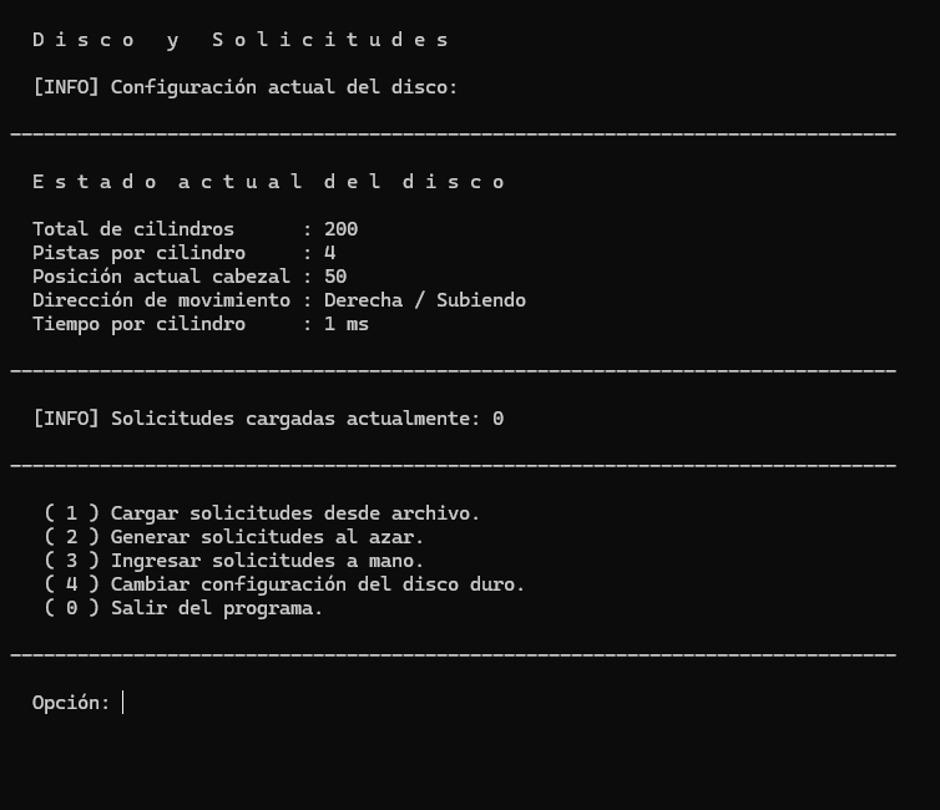
\includegraphics[width=1\linewidth]{1.jpeg}
    \end{center}

    \item \textbf{Configuración del Disco (Opción 4):}
    
    \begin{center}
        \textcolor{gray}{\textit{(Parámetros todos correctos)}}
        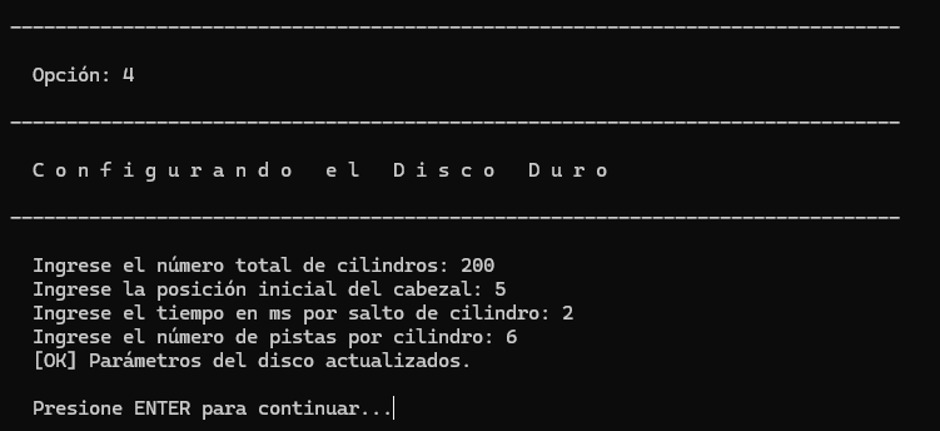
\includegraphics[width=1\linewidth]{2.jpeg}
        \end{center}

    \begin{center}
        \textcolor{gray}{\textit{(Parámetros con validación de datos ingresados)}}
        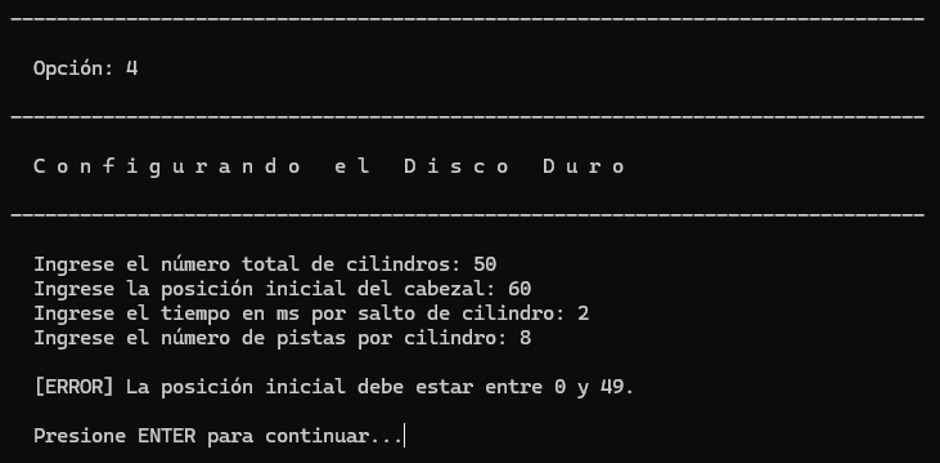
\includegraphics[width=1\linewidth]{3.jpeg}
    \end{center}

    \item \textbf{Impresión del Menú de Ejecución:}

    \begin{center}
        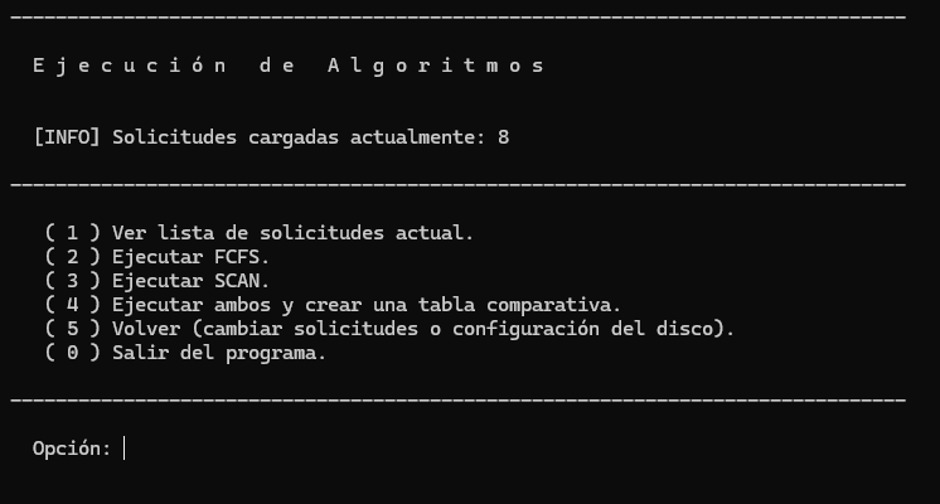
\includegraphics[width=1\linewidth]{4.jpeg}
    \end{center}

\newpage
    \item \textbf{Ejecución de SCAN (Opción 3):}
    
    \begin{center}
        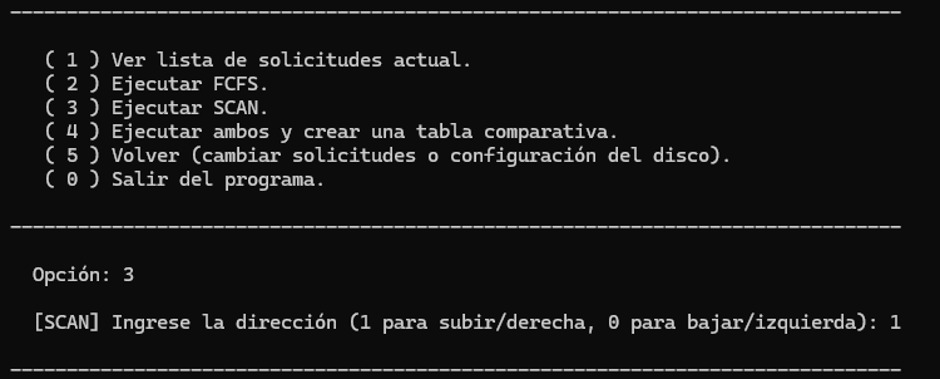
\includegraphics[width=1\linewidth]{5.jpeg}
    \end{center}
    
    \item \textbf{Tabla Comparativa (Opción 4):}
    
    \begin{center}
        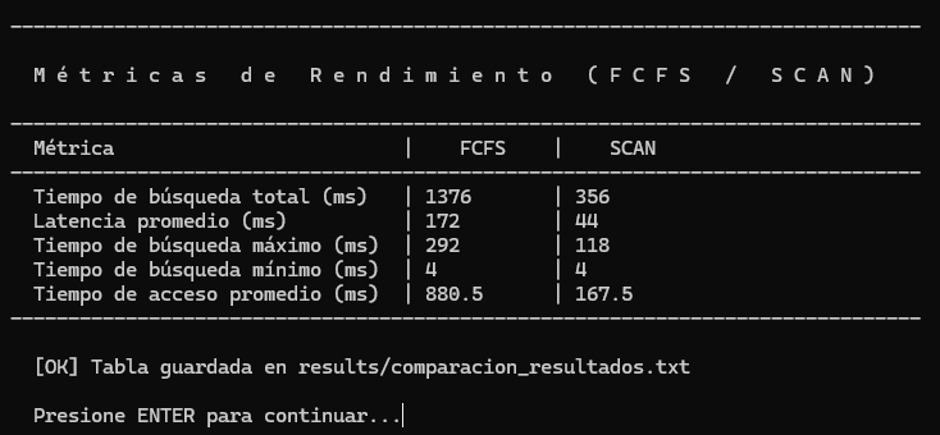
\includegraphics[width=1\linewidth]{6.jpeg}
    \end{center}
    
\end{enumerate}

\vfill

\section*{9. Casos de Prueba}

\textbf{Caso 1: Ejemplo clásico de libro}

\begin{itemize}
    \item Configuración del Disco (Menú 1, Opción 4): 200 cilindros, posición inicial 53, 1 ms por salto, 4 pistas.
    
    \begin{center}
        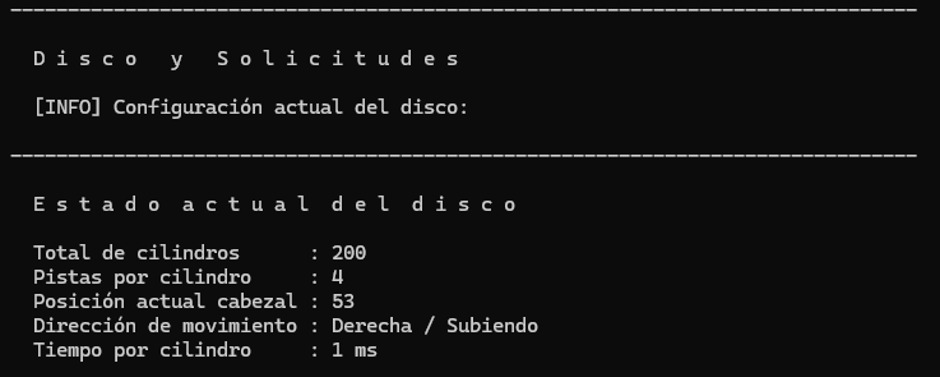
\includegraphics[width=1\linewidth]{7.jpeg}
    \end{center}
    
    \item Entrada de Datos (Menú 1, Opción 3): Ingreso manual de 8 solicitudes. Cilindros: 98, 183, 37, 122, 14, 124, 65, 67 (pista 0 para todas).

    \begin{center}
        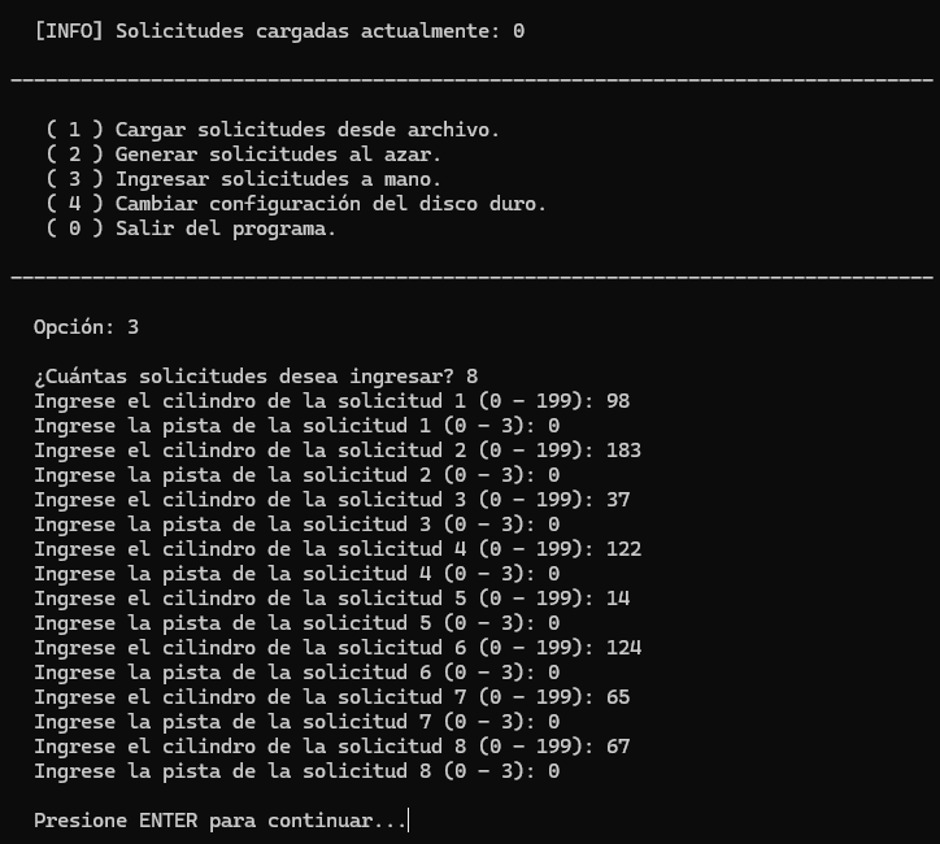
\includegraphics[width=1\linewidth]{8.jpeg}
    \end{center}
    
\end{itemize}

\newpage
\textit{Resultados Obtenidos:} FCFS mostrará un tiempo de búsqueda muy elevado debido a los saltos erráticos (ej. de 183 a 37). SCAN (iniciando hacia arriba, dirección 1) ordenará el barrido y reducirá drásticamente el tiempo total de movimiento y la latencia promedio.

    \begin{center}
        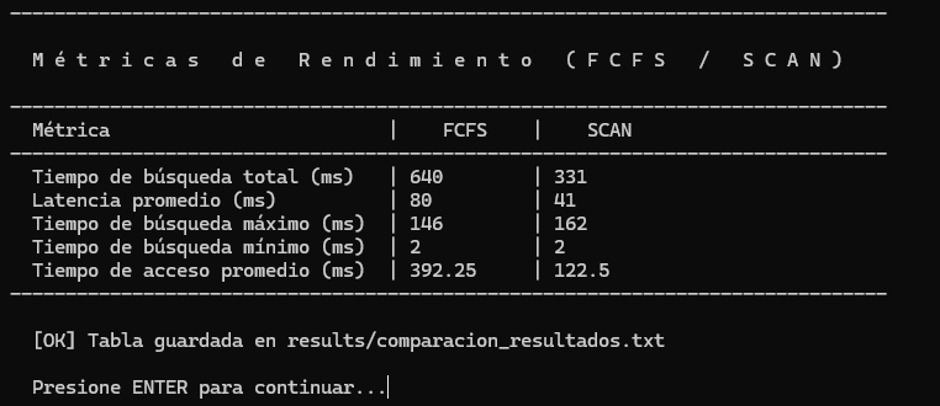
\includegraphics[width=1\linewidth]{9.jpeg}
    \end{center}

\textbf{Caso 2: Solicitudes aleatorias}

\begin{itemize}
    \item Configuración del Disco: Valores por defecto (200 cilindros, posición 50).

    \begin{center}
        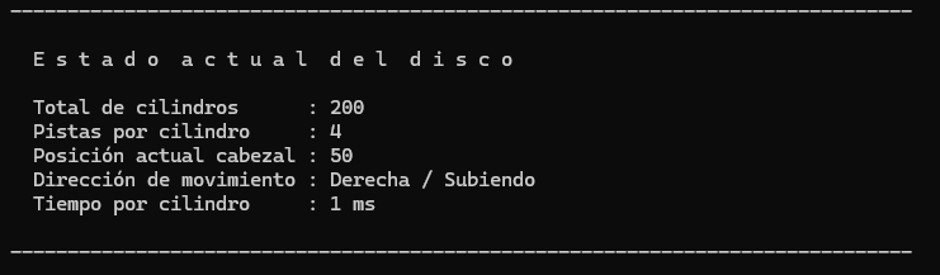
\includegraphics[width=1\linewidth]{10.jpeg}
    \end{center}

    \newpage
    \item Entrada de Datos (Menú 1, Opción 2): Generar 15 solicitudes al azar.

    \begin{center}
        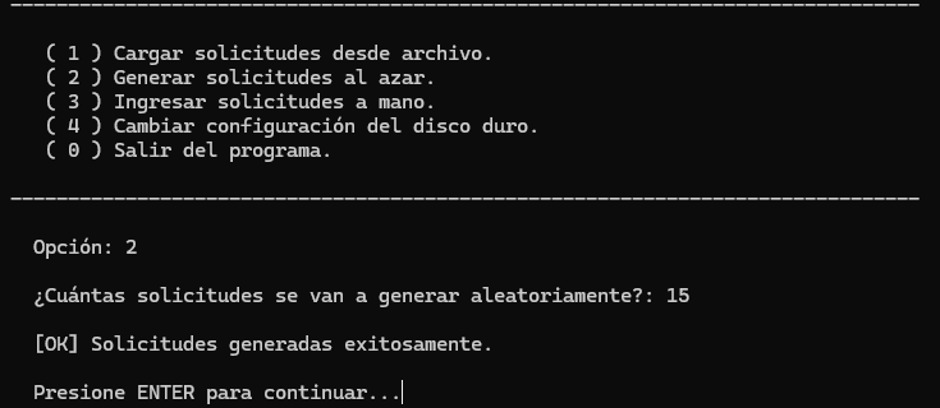
\includegraphics[width=1\linewidth]{11.jpeg}
    \end{center}
\end{itemize}

\textit{Resultados Obtenidos:} Al estar los datos altamente dispersos, el algoritmo FCFS penalizará severamente el tiempo de acceso acumulado. SCAN aprovechará el ordenamiento para optimizar el viaje físico del cabezal.

    \begin{center}
        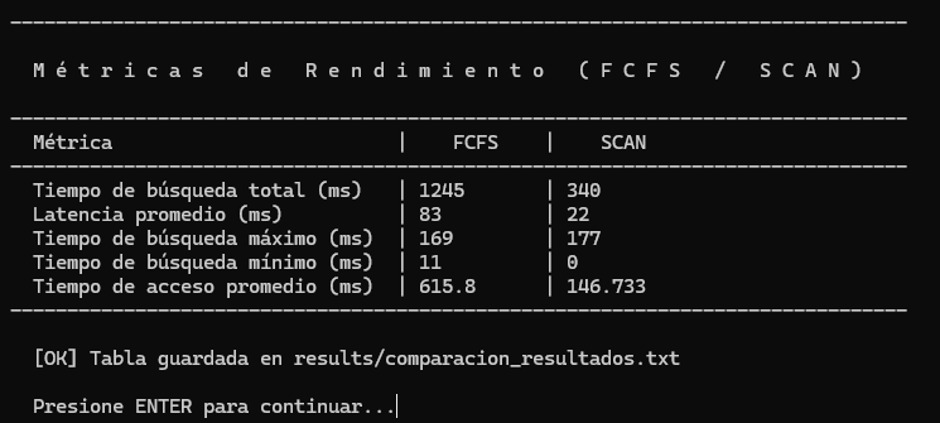
\includegraphics[width=1\linewidth]{12.jpeg}
    \end{center}

\newpage
\textbf{Caso 3: Todas las solicitudes de un solo lado}

\begin{itemize}
    \item Configuración del Disco (Menú 1, Opción 4): 200 cilindros, posición inicial 50.

    \begin{center}
        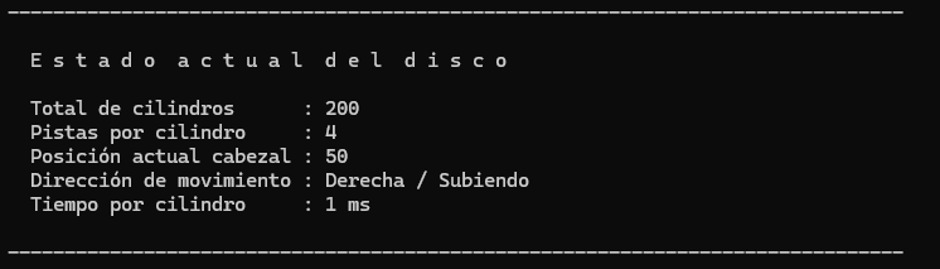
\includegraphics[width=1\linewidth]{13.jpeg}
    \end{center}
    
    \item Entrada de Datos (Menú 1, Opción 3): Ingreso manual exclusivo de cilindros mayores a 50 (ej. 70, 85, 110, 150, 190).

    \begin{center}
        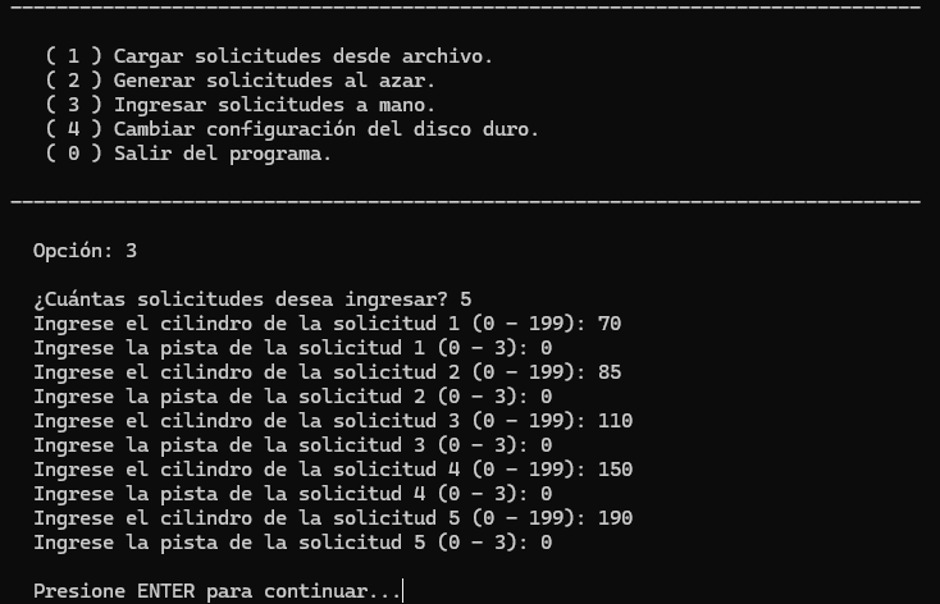
\includegraphics[width=1\linewidth]{14.jpeg}
    \end{center}
\end{itemize}

\newpage
\textit{Resultados Obtenidos:} Al ejecutar SCAN con dirección 1 (subiendo), el brazo atenderá todas las solicitudes. Como no hay peticiones a la izquierda (menores a 50), el algoritmo es lo suficientemente inteligente para detenerse y no tocar el extremo ni devolverse.

    \begin{center}
        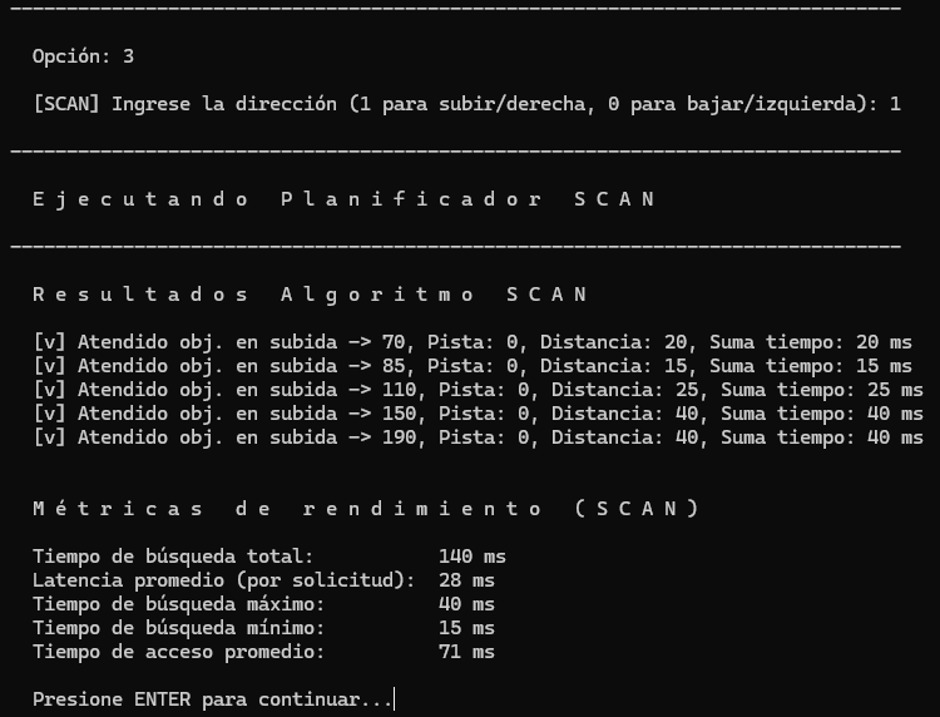
\includegraphics[width=1\linewidth]{15.jpeg}
    \end{center}

\newpage
\textbf{Caso 4: Cabezal en un extremo absoluto}

\begin{itemize}
    \item Configuración del Disco (Menú 1, Opción 4): 200 cilindros, posición inicial 0 (extremo inferior).

    \begin{center}
        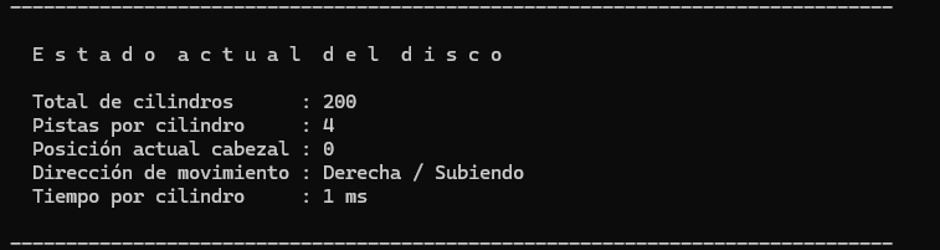
\includegraphics[width=1\linewidth]{16.jpeg}
    \end{center}
    
    \item Entrada de Datos: Manual (15, 45, 90, 130).

    \begin{center}
        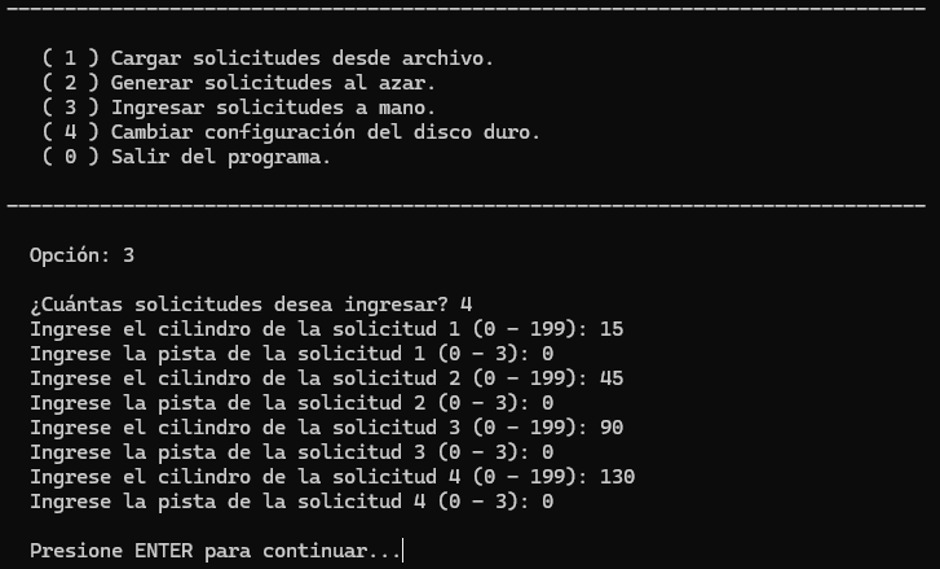
\includegraphics[width=1\linewidth]{17.jpeg}
    \end{center}
\end{itemize}

\newpage
\textit{Resultados Obtenidos:} El algoritmo SCAN (dirección 1) actuará como un barrido perfecto unidireccional.

    \begin{center}
        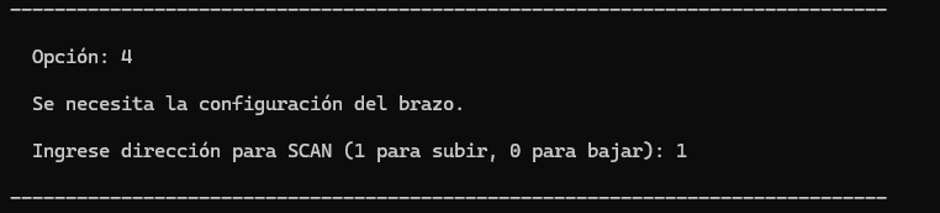
\includegraphics[width=1\linewidth]{18.jpeg}
    \end{center}
    \begin{center}
        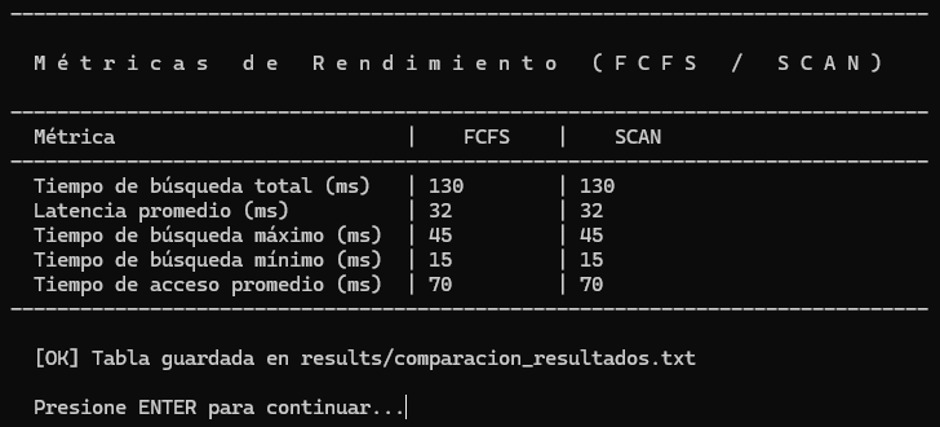
\includegraphics[width=1\linewidth]{19.jpeg}
    \end{center}

\newpage
\textbf{Otros casos probados: Solicitud en la posición actual}

\begin{itemize}
    \item Configuración del Disco: 200 cilindros, posición inicial 50.

    \begin{center}
        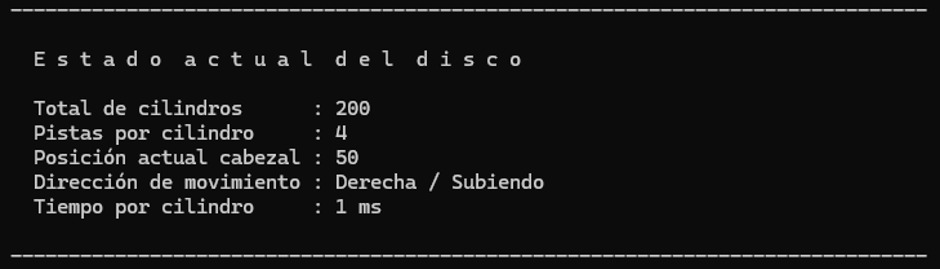
\includegraphics[width=1\linewidth]{20.jpeg}
    \end{center}
    
    \item Entrada de Datos (Menú 1, Opción 3): Ingreso manual incluyendo el cilindro donde ya está el cabezal (ej. 50, 80, 110).

    \begin{center}
        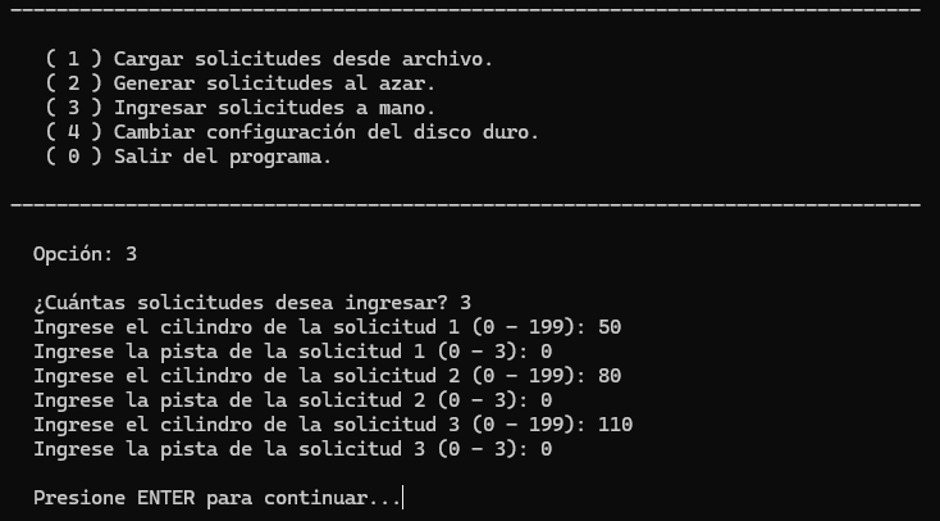
\includegraphics[width=1\linewidth]{21.jpeg}
    \end{center}
\end{itemize}

\newpage
\textit{Resultados Obtenidos:} El sistema detectará que la primera petición requiere 0 desplazamientos espaciales, resolviéndola de inmediato (0 ms).

    \begin{center}
        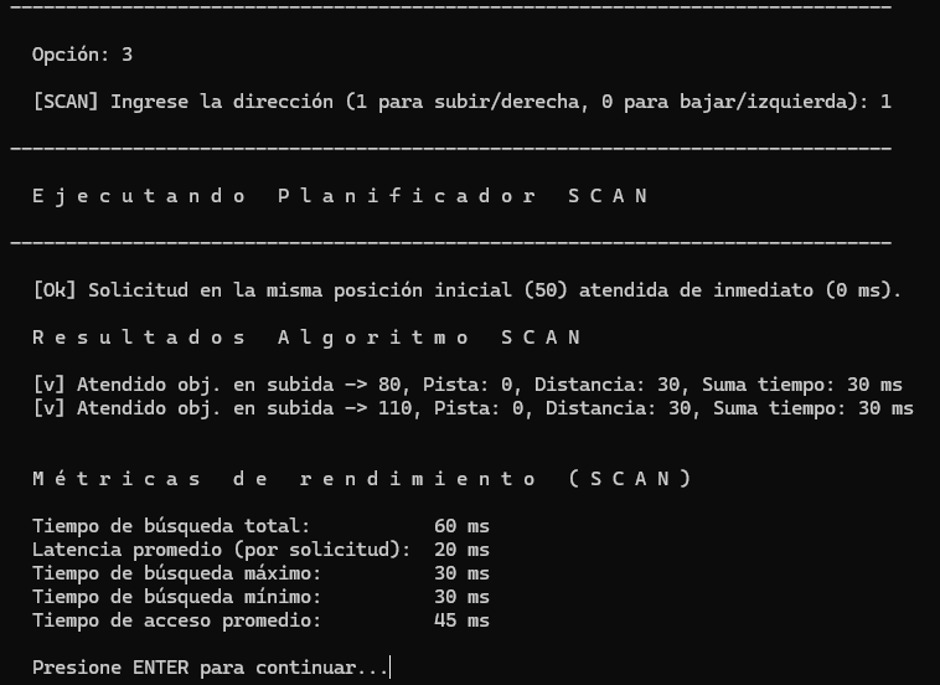
\includegraphics[width=1\linewidth]{22.jpeg}
    \end{center}

\vfill

\newpage
\section*{10. Análisis y Comparación de Resultados}

Una vez implementado el simulador y ejecutados los distintos casos de prueba, es posible realizar un análisis comparativo del comportamiento de los algoritmos FCFS y SCAN. Este análisis se basa tanto en las métricas cuantitativas generadas por el programa como en la observación del recorrido del cabezal en diferentes escenarios. A continuación se presentan los resultados obtenidos, el análisis por caso y las ventajas y desventajas observadas en la práctica.

\subsection*{10.2. Análisis por caso de prueba}

\textbf{Caso 1: Ejemplo clásico de libro}

En este escenario, FCFS presenta un rendimiento inferior debido a los cambios bruscos de dirección del cabezal. SCAN, al realizar un barrido ordenado, reduce tanto el tiempo total como la latencia promedio.
Se evidencia con claridad la ventaja de imponer un orden de recorrido frente a atender las solicitudes según su orden de llegada.

\textbf{Caso 2: Solicitudes aleatorias}

Cuando las solicitudes se encuentran altamente dispersas a lo largo del disco, la diferencia entre ambos algoritmos se vuelve más notoria. FCFS es severamente penalizado, ya que el cabezal realiza desplazamientos largos y sin criterio espacial. SCAN, al ordenar las peticiones y recorrer el disco de manera continua, optimiza el viaje físico del brazo y obtiene mejores métricas de tiempo total y tiempo de acceso promedio.

\newpage
\textbf{Caso 3: Todas las solicitudes de un solo lado}

En este caso se observa un comportamiento inteligente por parte de SCAN. Si todas las solicitudes se encuentran, por ejemplo, en cilindros mayores a la posición actual del cabezal y se elige la dirección ascendente, el algoritmo atiende todas las peticiones y finaliza sin necesidad de desplazarse hasta el extremo contrario ni de invertir la dirección. Esto demuestra que la implementación evita movimientos innecesarios cuando no existen solicitudes pendientes en el otro lado del disco.

\textbf{Caso 4: Cabezal ubicado en un extremo}

Cuando el cabezal inicia en el cilindro 0 y las solicitudes se encuentran distribuidas hacia valores mayores, SCAN con dirección ascendente se comporta como un recorrido unidireccional eficiente. En este escenario, la diferencia con FCFS sigue favoreciendo a SCAN, aunque la magnitud de la mejora depende de qué tan desordenadas se encuentren las solicitudes en el orden de llegada.

\textbf{Caso adicional: Solicitud en la posición actual del cabezal}

Cuando una de las solicitudes coincide con la posición inicial del cabezal, el sistema registra correctamente un tiempo de búsqueda de 0 ms para esa petición. Este comportamiento confirma que la lógica de cálculo de distancias funciona adecuadamente y que no se introducen costos artificiales cuando no existe desplazamiento real.

\subsection*{10.3. ¿En qué casos gana cada algoritmo?}

A partir de las pruebas realizadas, es posible establecer las siguientes conclusiones:

SCAN obtiene mejores resultados en la mayoría de los escenarios evaluados, especialmente cuando:

\begin{itemize}
    \item Las solicitudes se encuentran dispersas a lo largo del disco.
    \item Existen saltos grandes en el orden de llegada de las peticiones.
    \item Se busca reducir el tiempo total de búsqueda y la latencia promedio.
\end{itemize}

FCFS puede resultar aceptable únicamente en situaciones muy específicas, tales como:

\begin{itemize}
    \item Cuando las solicitudes ya llegan prácticamente ordenadas según la posición del cabezal.
    \item Cuando el número de solicitudes es muy pequeño.
    \item Cuando se prioriza la simplicidad y la equidad estricta por orden de llegada por encima del rendimiento.
\end{itemize}

En términos generales, SCAN demostró ser superior en los casos de prueba diseñados para este proyecto.

\subsection*{10.4. Ventajas y desventajas observadas}

\textbf{Algoritmo FCFS}

\textit{Ventajas observadas:}
\begin{itemize}
    \item Es simple de entender y de implementar.
    \item Garantiza que ninguna solicitud sea pospuesta indefinidamente, ya que respeta estrictamente el orden de llegada.
    \item Su comportamiento es predecible y fácil de rastrear.
\end{itemize}

\textit{Desventajas observadas:}
\begin{itemize}
    \item Genera tiempos de búsqueda elevados cuando las solicitudes están desordenadas.
    \item Produce recorridos erráticos del cabezal, con cambios frecuentes de dirección.
    \item Presenta una latencia promedio y un tiempo de acceso acumulado considerablemente mayores en la mayoría de las pruebas.
\end{itemize}

\textbf{Algoritmo SCAN}

\textit{Ventajas observadas:}
\begin{itemize}
    \item Reduce de forma notable el tiempo total de búsqueda y la latencia promedio.
    \item Evita los saltos largos e innecesarios al imponer un orden de recorrido.
    \item Se adapta de manera inteligente cuando todas las solicitudes se encuentran de un solo lado del cabezal.
    \item Ofrece un comportamiento más estable y eficiente en escenarios con solicitudes dispersas.
\end{itemize}

\textit{Desventajas observadas:}
\begin{itemize}
    \item Puede generar un tiempo de búsqueda máximo relativamente alto cuando debe recorrer hasta un extremo del disco antes de invertir la dirección.
    \item El rendimiento depende de la dirección inicial elegida; una elección inadecuada puede aumentar innecesariamente el recorrido.
    \item Su lógica de implementación es más compleja que la de FCFS.
\end{itemize}

\subsection*{10.5. Observaciones generales}

El análisis de los resultados permite confirmar que la planificación de discos tiene un impacto real y medible sobre el rendimiento del sistema. La diferencia de más de 180 ms en el tiempo total de búsqueda entre FCFS y SCAN, observada en el caso clásico, evidencia que la elección del algoritmo no es un detalle menor, sino un factor determinante en la eficiencia del acceso a almacenamiento secundario.

Asimismo, el simulador demostró ser una herramienta útil para visualizar el comportamiento interno de cada algoritmo, ya que entrega métricas numéricas, y también el detalle del recorrido del cabezal.

\vfill

\section*{11. Conclusiones}

El desarrollo del presente proyecto permitió diseñar, implementar y evaluar un simulador de planificación de discos orientado al estudio de los algoritmos FCFS y SCAN, en el marco de la asignatura de Arquitectura del Computador. A lo largo del trabajo se integraron conceptos teóricos fundamentales con una solución práctica desarrollada en C++, logrando construir una herramienta funcional, modular y capaz de generar métricas cuantitativas para el análisis comparativo de ambas políticas de planificación.

En primer lugar, se logró modelar de manera adecuada el comportamiento básico de un disco duro, representando sus principales componentes y parámetros: el número de cilindros, la posición del cabezal, la dirección de movimiento, el tiempo de desplazamiento entre cilindros y la cantidad de pistas por cilindro. Este modelado constituyó la base sobre la cual fue posible simular el costo real de cada movimiento del brazo lector y, por consiguiente, evaluar el impacto de distintos órdenes de atención de las solicitudes.

En segundo lugar, se implementaron de forma correcta los algoritmos FCFS y SCAN, junto con un conjunto de métricas de rendimiento que incluyen el tiempo total de búsqueda, la latencia promedio, los tiempos máximo y mínimo de búsqueda, y el tiempo de acceso promedio acumulado. La generación automática de archivos de resultados facilitó el análisis posterior y permitió conservar evidencia clara de cada experimentación realizada.

Desde el punto de vista del usuario, se construyó una interfaz de consola estructurada en dos menús complementarios, la cual permite configurar el disco, cargar solicitudes de distintas maneras (archivo, generación aleatoria o ingreso manual), ejecutar los algoritmos de forma individual o comparativa y visualizar los resultados de manera ordenada. Esta organización hizo posible que el proceso de prueba fuera sistemático y reproducible.

Los resultados experimentales obtenidos confirmaron las diferencias teóricas existentes entre ambos algoritmos. En el caso clásico de libro, SCAN redujo el tiempo total de búsqueda de 535 ms a 348 ms y la latencia promedio de 66 ms a 43 ms, evidenciando una mejora sustancial respecto a FCFS. De manera general, se observó que SCAN ofrece un mejor rendimiento cuando las solicitudes se encuentran dispersas o desordenadas, mientras que FCFS tiende a generar recorridos erráticos y costos más elevados. Asimismo, se comprobó que SCAN es capaz de evitar movimientos innecesarios cuando todas las solicitudes se ubican de un solo lado del cabezal, y que el sistema registra correctamente un tiempo de búsqueda nulo cuando una solicitud coincide con la posición actual del brazo.

El desarrollo del proyecto también permitió consolidar aprendizajes importantes. Desde la perspectiva teórica, se comprendió con mayor profundidad por qué la planificación de discos constituye un problema relevante dentro de la arquitectura de computadores: el tiempo de búsqueda del cabezal sigue siendo un factor crítico en el rendimiento de las operaciones de entrada y salida.

Desde la perspectiva práctica, se reforzaron habilidades de programación en C++, diseño modular, uso de la biblioteca estándar, manejo de archivos, validación de entradas y automatización de la compilación mediante Makefile. Además, se adquirió experiencia en la construcción de una herramienta de simulación orientada al análisis experimental, lo cual implica además de escribir código funcional, diseñar casos de prueba, interpretar métricas y elaborar conclusiones fundamentadas.

Otro aprendizaje significativo fue la importancia de la organización del software. La separación del proyecto en archivos de cabecera, archivos fuente, datos de entrada y resultados de salida facilitó tanto el desarrollo en equipo como la comprensión del sistema como un conjunto de módulos interrelacionados. De igual forma, la necesidad de validar entradas, controlar casos borde y presentar resultados claros demostró que un programa de simulación no puede limitarse a implementar un algoritmo, sino que debe considerar la experiencia de uso y la confiabilidad de los datos generados.

Como trabajo futuro, se plantea la posibilidad de ampliar el simulador mediante la incorporación de nuevos algoritmos de planificación, la inclusión de métricas adicionales, el uso de trazas de solicitudes reales y el desarrollo de una interfaz visual que permita observar de forma dinámica el recorrido del brazo sobre el disco. También resultaría de interés comparar el comportamiento de los algoritmos bajo distintas distribuciones estadísticas de solicitudes y analizar su impacto en escenarios de mayor escala.

En definitiva, el proyecto no solo permitió construir una herramienta funcional para la simulación de algoritmos de planificación de discos, sino que también consolidó una comprensión integral del problema abordado. A través de la combinación de fundamentos teóricos, implementación práctica y análisis experimental, se evidenció que la forma en que se ordenan las solicitudes de acceso a disco tiene un efecto concreto y medible sobre el rendimiento del sistema. De este modo, el trabajo realizado contribuye a reforzar la importancia de la gestión eficiente de las operaciones de entrada y salida dentro del estudio de la Arquitectura de Computadores.

\end{document}